\chapter{Attosecond Transient-absorption Spectroscopy}
\label{chap:ATS}

\section{Introduction}
\label{sec:intro_ats}

\section{Theory}
\label{sec:atas_theory}

\section{Fano resonances in Argon}
\label{sec:fano_ar}

\begin{table}[]
	\centering
	\begin{tabular}{lcccc}
		\hline\hline
		\multicolumn{1}{c}{} & $\Delta E$ [eV]   & $\Gamma$ [meV]   & $q$         & $\rho^2$     \\ \hline
		$3s3p^64p$              & 26.605 & 80.2(7) & -0.286(4) & 0.840(3) \\
		$3s3p^65p$              & 27.994 & 28.5(8) & -0.177(3) & 0.848(3) \\
		$3s3p^66p$              & 28.509 & 12.2(3) & -0.135(9) & 0.852(9) \\
		$3s3p^67p$              & 28.757 & 6.6(1)  & -0.125(4) & 0.846(9) \\
		$3s3p^68p$              & 28.898 & 4.5(2)  & -0.132(4) & 0.77(2)  \\ \hline\hline
	\end{tabular}
	\caption{Paramters of the $3s3p^6np$ Fano resonances in argon. These values were extracted from experimental cross sections, see \cite{caretteMulticonfigurationalHartreeFockClosecoupling2013}.}
	\label{table:fano_params}
\end{table}

\begin{figure}
	\centering
	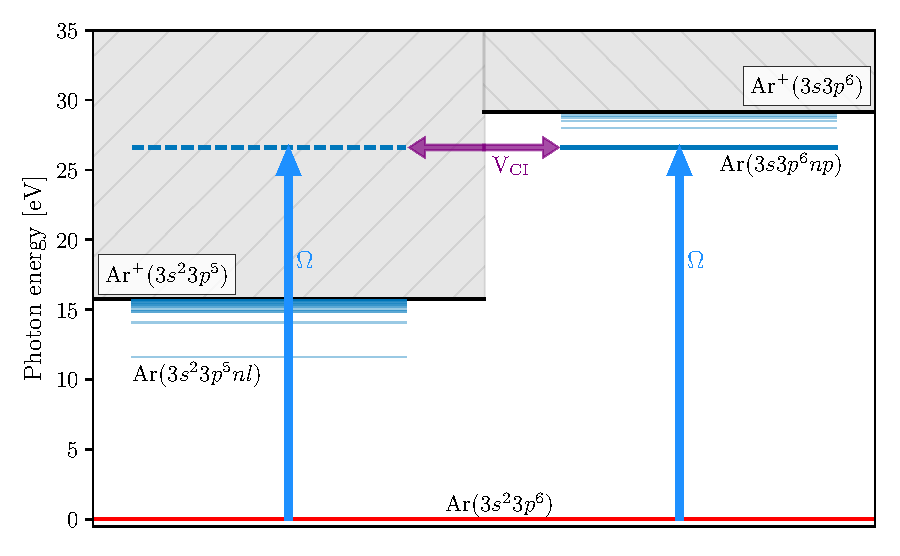
\includegraphics[width=0.8\textwidth]{figures/ATS/fano_level_diagram.pdf}
	\caption{Incomplete level diagram}
	\label{fig:fano_level_diagram}
\end{figure}

\begin{figure}
	\centering
	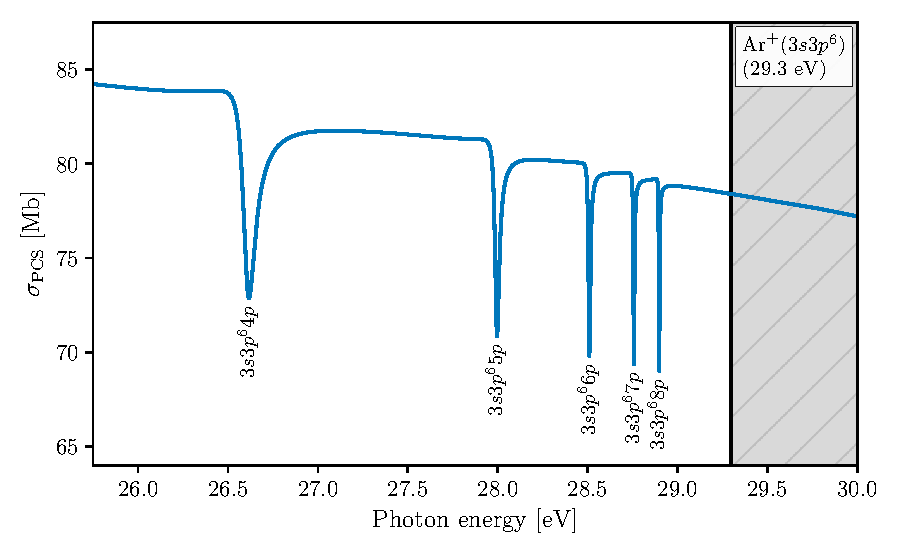
\includegraphics[width=0.8\textwidth]{figures/ATS/fano_GS.pdf}
	\caption{Photoabsorption cross section of the Argon $3s3p^6np$ Fano resonances (blue curve), with only resonances up to $n=8$ shown.  Grey shaded area indicates the energetic region above the $\mathrm{Ar}^+(3s3p^6)$ ionization threshold. Values used to calculate this cross section are shown in Table \ref{table:fano_params}.}
	\label{fig:fano_gs_pcs}
\end{figure}


\section{Strong-field Transient Absorption in Argon}
\label{sec:ATS_ar}

\subsection{Experimental setup}
\label{sec:ATS_ar_exp_setup}

\subsection{Results}
\label{sec:ATS_ar_results}

\section{Conculsion}
\label{sec:ATS_conclusion}

